\documentclass[aspectratio=169]{beamer}
\usepackage[utf8]{inputenc}
\usepackage[T1]{fontenc}
\usepackage[brazil]{babel}
\usepackage{ragged2e}
\usepackage{booktabs}
\usepackage{verbatim}
\usetheme{AnnArbor}
\usecolortheme{orchid}
\usefonttheme[onlymath]{serif}
\usepackage{listings}
\usepackage{colortbl	}
\usepackage{array}

\newcolumntype{C}[0]{>{\centering\arraybackslash}p{0.4cm}}

\lstset{language=C++,
	backgroundcolor=\color{green!10},
	basicstyle=\ttfamily,
	keywordstyle=\color{blue}\ttfamily,
	stringstyle=\color{red}\ttfamily,
	commentstyle=\color{green}\ttfamily,
	morecomment=[l][\color{magenta}]{\#}
}

\AtBeginSection[]{
  \begin{frame}
  \vfill
  \centering
  \begin{beamercolorbox}[sep=8pt,center,shadow=true,rounded=true]{title}
    \usebeamerfont{title}\insertsectionhead\par%
  \end{beamercolorbox}
  \vfill
  \end{frame}
}

\title[\sc{Algoritmos de Ordenação}]{Algoritmos de Ordenação}
\author[Roland Teodorowitsch]{Roland Teodorowitsch}
\institute[ALEST I - EP - PUCRS]{Algoritmos e Estruturas de Dados I - Escola Politécnica - PUCRS}
\date{22 de agosto de 2023}

\begin{document}
\justifying

%-------------------------------------------------------
\begin{frame}
	\titlepage
\end{frame}

%=======================================================
\section{Introdução}

%-------------------------------------------------------
\begin{frame}\frametitle{Leitura(s) Recomendada(s)}

\begin{columns}[T]
\begin{column}{0.15\linewidth}
\vspace{-3mm}
\begin{figure}[h]
	\centering
	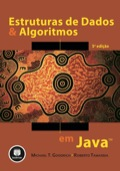
\includegraphics[height=0.3\paperheight]{imagens/livro_goodrich.jpg}
\end{figure}
\end{column}
\begin{column}{0.85\linewidth}
\vspace{3mm}
\textbf{Seções 3.1.2, 11.1 (\emph{Merge Sort}), 11.2 (\emph{Quick Sort}), 11.3.3 (comparação)}\\
\scriptsize{GOODRICH, Michael T.; TAMASSIA, Roberto. \textbf{Estruturas de dados e algoritmos em Java}. Tradução: Bernardo Copstein. 5. ed. Porto Alegre: Bookman, 2013. xxii, 713 p. E-book. ISBN 9788582600191. Tradução de: Data Structures and Algorithms in Java, 5th Edition. Disponível em: \textless{}\url{https://integrada.minhabiblioteca.com.br/\#/books/9788582600191/}\textgreater{}. Acesso em: 01 ago. 2023.}
\end{column}
\end{columns}

\end{frame}

%-------------------------------------------------------
\begin{frame}\frametitle{Sites sobre Ordenação [*]}
\begin{itemize}
{\small
	\item Animações:\\\url{http://www.sorting-algorithms.com/}
	\item Algoritmos na wikipedia:\\\url {https://en.wikipedia.org/wiki/Sorting_algorithm}
	\item Danças:\\\url{http://makezine.com/2011/04/12/data-sorting-dances/}
	\item 15 algoritmos em 6 minutos:\\\url{https://www.youtube.com/watch?v=kPRA0W1kECg}
	\item Visualização e comparação de algoritmos de ordenação:\\\url{https://www.youtube.com/watch?v=ZZuD6iUe3Pc}
	\item Visualização \emph{Bubble Sort vs Quick Sort}:\\\url{https://www.youtube.com/watch?v=aXXWXz5rF64}
	\item Visualização \emph{Merge Sort vs Quick Sort}:\\\url{https://www.youtube.com/watch?v=es2T6KY45cA}
}
\end{itemize}
\end{frame}

%-------------------------------------------------------
\begin{frame}\frametitle{Revisão: Algoritmos de Pesquisa}
\begin{itemize}
	\item Pesquisa Linear
	\begin{itemize}
		\item Pode ser aplicada sobre qualquer coleção, ordenada ou não
		\item Procura um item, comparando-o com cada elemento da coleção, até achar ou chegar no final
		\item Melhor caso: o item procurado está na primeira posição da coleção
		\item Pior caso: o item NÃO está na coleção
		\item Complexidade: $O(n)$
	\end{itemize}
	\item Pesquisa Binária
	\begin{itemize}
		\item A coleção deve estar ordenada
		\item Estratégia básica:
		\begin{itemize}
			\item Verifica o elemento central: se encontrou, a busca termina
			\item Se o item for menor que o central, considera apenas a parte abaixo do elemento central
			\item Se o item for maior que o central, considera apenas a parte acima do elemento central
		\end{itemize}
		\item Trabalha subdividindo a coleção e reaplicando sempre a estratégia básica, o que o torna adequado para implementação recursiva
		\item Complexidade: $O(\log n)$
	\end{itemize}
\end{itemize}
\end{frame}

%=======================================================
\section{Algoritmos de Ordenação}

%-------------------------------------------------------
\begin{frame}\frametitle{Algoritmos de Ordenação}
\begin{itemize}
	\item Organizam os elementos de uma coleção segundo determinado critério (ordem crescente de valor, por exemplo)
	\item Operação básica: troca de elementos
	\item Exemplos
	\begin{itemize}
		\item \emph{Bubble Sort}
		\item \emph{Selection Sort}
		\item \emph{Insertion Sort}
		\item \emph{Merge Sort}
		\item \emph{Quick Sort}
		\item etc.
	\end{itemize}
	\item Em geral, os mais simples nem sempre tem bom desempenho (menos otimizados)
	\item Algoritmos com bom desempenho costumam ser mais sofisticados
	\item São importantes quando se quer implementar busca eficiente (pesquisa binária)
\end{itemize}
\end{frame}

%=======================================================
\section{\emph{Bubble Sort}}

%-------------------------------------------------------
\begin{frame}\frametitle{\emph{Bubble Sort}}
\begin{itemize}
	\item É um dos métodos mais simples de ordenação
	\item Estratégia: compara elementos adjacentes, e, se estiverem fora de ordem, troca os elementos
	\item Repete-se a estratégia básica até que a coleção esteja ordenada
	\item Complexidade: $O(n)$ (melhor caso) ou $O(n^2)$ (pior caso)
\end{itemize}
\end{frame}

%-------------------------------------------------------
\begin{frame}\frametitle{\emph{Bubble Sort}: Exemplo}
\begin{center}
\begin{tabular}{CCCCCCCCCC}
\tiny{0} & \tiny{1} & \tiny{2} & \tiny{3} & \tiny{4} & \tiny{5} & \tiny{6} & \tiny{7} & \tiny{8} & \tiny{9}\\
\hline
\multicolumn{1}{|C|}{5} & \multicolumn{1}{|C|}{7} & \multicolumn{1}{|C|}{8} & \multicolumn{1}{|C|}{1} & \multicolumn{1}{|C|}{10} & \multicolumn{1}{|C|}{9} & \multicolumn{1}{|C|}{4} & \multicolumn{1}{|C|}{6} & \multicolumn{1}{|C|}{3} & \multicolumn{1}{|C|}{2}\\
\hline
\hline
\multicolumn{1}{|C|}{5} & \multicolumn{1}{|C|}{7} & \multicolumn{1}{|C|}{1} & \multicolumn{1}{|C|}{8} & \multicolumn{1}{|C|}{9} & \multicolumn{1}{|C|}{4} & \multicolumn{1}{|C|}{6} & \multicolumn{1}{|C|}{3} & \multicolumn{1}{|C|}{2} & \multicolumn{1}{|C|}{\cellcolor{green}10}\\
\hline
\hline
\multicolumn{1}{|C|}{5} & \multicolumn{1}{|C|}{1} & \multicolumn{1}{|C|}{7} & \multicolumn{1}{|C|}{8} & \multicolumn{1}{|C|}{4} & \multicolumn{1}{|C|}{6} & \multicolumn{1}{|C|}{3} & \multicolumn{1}{|C|}{2} & \multicolumn{1}{|C|}{\cellcolor{green}9} & \multicolumn{1}{|C|}{\cellcolor{green}10}\\
\hline
\hline
\multicolumn{1}{|C|}{1} & \multicolumn{1}{|C|}{5} & \multicolumn{1}{|C|}{7} & \multicolumn{1}{|C|}{4} & \multicolumn{1}{|C|}{6} & \multicolumn{1}{|C|}{3} & \multicolumn{1}{|C|}{2} & \multicolumn{1}{|C|}{\cellcolor{green}8} & \multicolumn{1}{|C|}{\cellcolor{green}9} & \multicolumn{1}{|C|}{\cellcolor{green}10}\\
\hline
\hline
\multicolumn{1}{|C|}{1} & \multicolumn{1}{|C|}{5} & \multicolumn{1}{|C|}{4} & \multicolumn{1}{|C|}{6} & \multicolumn{1}{|C|}{3} & \multicolumn{1}{|C|}{2} & \multicolumn{1}{|C|}{\cellcolor{green}7} & \multicolumn{1}{|C|}{\cellcolor{green}8} & \multicolumn{1}{|C|}{\cellcolor{green}9} & \multicolumn{1}{|C|}{\cellcolor{green}10}\\
\hline
\hline
\multicolumn{1}{|C|}{1} & \multicolumn{1}{|C|}{4} & \multicolumn{1}{|C|}{5} & \multicolumn{1}{|C|}{3} & \multicolumn{1}{|C|}{2} & \multicolumn{1}{|C|}{\cellcolor{green}6} & \multicolumn{1}{|C|}{\cellcolor{green}7} & \multicolumn{1}{|C|}{\cellcolor{green}8} & \multicolumn{1}{|C|}{\cellcolor{green}9} & \multicolumn{1}{|C|}{\cellcolor{green}10}\\
\hline
\hline
\multicolumn{1}{|C|}{1} & \multicolumn{1}{|C|}{4} & \multicolumn{1}{|C|}{3} & \multicolumn{1}{|C|}{2} & \multicolumn{1}{|C|}{\cellcolor{green}5} & \multicolumn{1}{|C|}{\cellcolor{green}6} & \multicolumn{1}{|C|}{\cellcolor{green}7} & \multicolumn{1}{|C|}{\cellcolor{green}8} & \multicolumn{1}{|C|}{\cellcolor{green}9} & \multicolumn{1}{|C|}{\cellcolor{green}10}\\
\hline
\hline
\multicolumn{1}{|C|}{1} & \multicolumn{1}{|C|}{3} & \multicolumn{1}{|C|}{2} & \multicolumn{1}{|C|}{\cellcolor{green}4} & \multicolumn{1}{|C|}{\cellcolor{green}5} & \multicolumn{1}{|C|}{\cellcolor{green}6} & \multicolumn{1}{|C|}{\cellcolor{green}7} & \multicolumn{1}{|C|}{\cellcolor{green}8} & \multicolumn{1}{|C|}{\cellcolor{green}9} & \multicolumn{1}{|C|}{\cellcolor{green}10}\\
\hline
\hline
\multicolumn{1}{|C|}{1} & \multicolumn{1}{|C|}{2} & \multicolumn{1}{|C|}{\cellcolor{green}3} & \multicolumn{1}{|C|}{\cellcolor{green}4} & \multicolumn{1}{|C|}{\cellcolor{green}5} & \multicolumn{1}{|C|}{\cellcolor{green}6} & \multicolumn{1}{|C|}{\cellcolor{green}7} & \multicolumn{1}{|C|}{\cellcolor{green}8} & \multicolumn{1}{|C|}{\cellcolor{green}9} & \multicolumn{1}{|C|}{\cellcolor{green}10}\\
\hline
\hline
\multicolumn{1}{|C|}{\cellcolor{green}1} & \multicolumn{1}{|C|}{\cellcolor{green}2} & \multicolumn{1}{|C|}{\cellcolor{green}3} & \multicolumn{1}{|C|}{\cellcolor{green}4} & \multicolumn{1}{|C|}{\cellcolor{green}5} & \multicolumn{1}{|C|}{\cellcolor{green}6} & \multicolumn{1}{|C|}{\cellcolor{green}7} & \multicolumn{1}{|C|}{\cellcolor{green}8} & \multicolumn{1}{|C|}{\cellcolor{green}9} & \multicolumn{1}{|C|}{\cellcolor{green}10}\\
\hline
\end{tabular}
\end{center}
\end{frame}	

%-------------------------------------------------------
\begin{frame}[fragile]\frametitle{\emph{Bubble Sort}: Implementação}
\lstinputlisting[basicstyle=\ttfamily\small]{src/bubbleSort.cpp}
\end{frame}

%-------------------------------------------------------
\begin{frame}[fragile]\frametitle{\emph{Bubble Sort}: Mais informações [*]}
\begin{itemize}
	\item \url{http://www.sorting-algorithms.com/bubble-sort}
	\item \url{https://www.hackerearth.com/practice/algorithms/sorting/bubble-sort/tutorial/}
\end{itemize}
\end{frame}

%=======================================================
\section{\emph{Selection Sort}}

%-------------------------------------------------------
\begin{frame}\frametitle{\emph{Selection Sort}}
\begin{itemize}
	\item É um algorimo de ordenação por seleção
	\item Fácil de implementar e bastante intuitivo, o que não garante eficiência...
	\item Estratégia: procurar o menor elemento e colocá-lo na sua posiçao
	\item Repete-se a estratégia até que todos os elementos estejam em sua posição
	\item Complexidade: $O(n^2)$ (melhor e pior caso)
\end{itemize}
\end{frame}

%-------------------------------------------------------
\begin{frame}\frametitle{\emph{Selection Sort}: Exemplo}
\begin{center}
\begin{tabular}{CCCCCCCCCC}
\tiny{0} & \tiny{1} & \tiny{2} & \tiny{3} & \tiny{4} & \tiny{5} & \tiny{6} & \tiny{7} & \tiny{8} & \tiny{9}\\
\hline
\multicolumn{1}{|C|}{5} & \multicolumn{1}{|C|}{7} & \multicolumn{1}{|C|}{8} & \multicolumn{1}{|C|}{1} & \multicolumn{1}{|C|}{10} & \multicolumn{1}{|C|}{9} & \multicolumn{1}{|C|}{4} & \multicolumn{1}{|C|}{6} & \multicolumn{1}{|C|}{3} & \multicolumn{1}{|C|}{2}\\
\hline
\hline
\multicolumn{1}{|C|}{\cellcolor{green}1} & \multicolumn{1}{|C|}{7} & \multicolumn{1}{|C|}{8} & \multicolumn{1}{|C|}{5} & \multicolumn{1}{|C|}{10} & \multicolumn{1}{|C|}{9} & \multicolumn{1}{|C|}{4} & \multicolumn{1}{|C|}{6} & \multicolumn{1}{|C|}{3} & \multicolumn{1}{|C|}{2}\\
\hline
\hline
\multicolumn{1}{|C|}{\cellcolor{green}1} & \multicolumn{1}{|C|}{\cellcolor{green}2} & \multicolumn{1}{|C|}{8} & \multicolumn{1}{|C|}{5} & \multicolumn{1}{|C|}{10} & \multicolumn{1}{|C|}{9} & \multicolumn{1}{|C|}{4} & \multicolumn{1}{|C|}{6} & \multicolumn{1}{|C|}{3} & \multicolumn{1}{|C|}{7}\\
\hline
\hline
\multicolumn{1}{|C|}{\cellcolor{green}1} & \multicolumn{1}{|C|}{\cellcolor{green}2} & \multicolumn{1}{|C|}{\cellcolor{green}3} & \multicolumn{1}{|C|}{5} & \multicolumn{1}{|C|}{10} & \multicolumn{1}{|C|}{9} & \multicolumn{1}{|C|}{4} & \multicolumn{1}{|C|}{6} & \multicolumn{1}{|C|}{8} & \multicolumn{1}{|C|}{7}\\
\hline
\hline
\multicolumn{1}{|C|}{\cellcolor{green}1} & \multicolumn{1}{|C|}{\cellcolor{green}2} & \multicolumn{1}{|C|}{\cellcolor{green}3} & \multicolumn{1}{|C|}{\cellcolor{green}4} & \multicolumn{1}{|C|}{10} & \multicolumn{1}{|C|}{9} & \multicolumn{1}{|C|}{5} & \multicolumn{1}{|C|}{6} & \multicolumn{1}{|C|}{8} & \multicolumn{1}{|C|}{7}\\
\hline
\hline
\multicolumn{1}{|C|}{\cellcolor{green}1} & \multicolumn{1}{|C|}{\cellcolor{green}2} & \multicolumn{1}{|C|}{\cellcolor{green}3} & \multicolumn{1}{|C|}{\cellcolor{green}4} & \multicolumn{1}{|C|}{\cellcolor{green}5} & \multicolumn{1}{|C|}{9} & \multicolumn{1}{|C|}{10} & \multicolumn{1}{|C|}{6} & \multicolumn{1}{|C|}{8} & \multicolumn{1}{|C|}{7}\\
\hline
\hline
\multicolumn{1}{|C|}{\cellcolor{green}1} & \multicolumn{1}{|C|}{\cellcolor{green}2} & \multicolumn{1}{|C|}{\cellcolor{green}3} & \multicolumn{1}{|C|}{\cellcolor{green}4} & \multicolumn{1}{|C|}{\cellcolor{green}5} & \multicolumn{1}{|C|}{\cellcolor{green}6} & \multicolumn{1}{|C|}{10} & \multicolumn{1}{|C|}{9} & \multicolumn{1}{|C|}{8} & \multicolumn{1}{|C|}{7}\\
\hline
\hline
\multicolumn{1}{|C|}{\cellcolor{green}1} & \multicolumn{1}{|C|}{\cellcolor{green}2} & \multicolumn{1}{|C|}{\cellcolor{green}3} & \multicolumn{1}{|C|}{\cellcolor{green}4} & \multicolumn{1}{|C|}{\cellcolor{green}5} & \multicolumn{1}{|C|}{\cellcolor{green}6} & \multicolumn{1}{|C|}{\cellcolor{green}7} & \multicolumn{1}{|C|}{9} & \multicolumn{1}{|C|}{8} & \multicolumn{1}{|C|}{10}\\
\hline
\hline
\multicolumn{1}{|C|}{\cellcolor{green}1} & \multicolumn{1}{|C|}{\cellcolor{green}2} & \multicolumn{1}{|C|}{\cellcolor{green}3} & \multicolumn{1}{|C|}{\cellcolor{green}4} & \multicolumn{1}{|C|}{\cellcolor{green}5} & \multicolumn{1}{|C|}{\cellcolor{green}6} & \multicolumn{1}{|C|}{\cellcolor{green}7} & \multicolumn{1}{|C|}{\cellcolor{green}8} & \multicolumn{1}{|C|}{9} & \multicolumn{1}{|C|}{10}\\
\hline
\hline
\multicolumn{1}{|C|}{\cellcolor{green}1} & \multicolumn{1}{|C|}{\cellcolor{green}2} & \multicolumn{1}{|C|}{\cellcolor{green}3} & \multicolumn{1}{|C|}{\cellcolor{green}4} & \multicolumn{1}{|C|}{\cellcolor{green}5} & \multicolumn{1}{|C|}{\cellcolor{green}6} & \multicolumn{1}{|C|}{\cellcolor{green}7} & \multicolumn{1}{|C|}{\cellcolor{green}8} & \multicolumn{1}{|C|}{\cellcolor{green}9} & \multicolumn{1}{|C|}{\cellcolor{green}10}\\
\hline
\end{tabular}
\end{center}
\end{frame}

%-------------------------------------------------------
\begin{frame}\frametitle{\emph{Selection Sort}: Implementação}
\lstinputlisting[basicstyle=\ttfamily\small]{src/selectionSort.cpp}
\end{frame}

%=======================================================
\section{\emph{Insertion Sort}}

%-------------------------------------------------------
\begin{frame}\frametitle{\emph{Insertion Sort}}
\begin{itemize}
	\item É um algorimo de ordenação por inserção
	\item Estratégia:
	\begin{itemize}
		\item Escolhe-se uma base que inicia no segundo elemento e avança até o último elemento
		\item Sempre à esquerda da base todos os elementos devem estar ordenados
		\item Busca-se a posição da base nos elementos à esquerda, sempre deslocando os elementos uma posição para a direita enquanto não chegar na posição correta da base
		\item Quando chegar na posição correta da base, atribui-se o valor da base para esta posição
	\end{itemize}
	\item Trata-se de uma algoritmo um pouco mais avançado do que os dois anteriores
	\item Complexidade: $O(n)$ (melhor caso) ou $O(n^2)$ (pior caso)
\end{itemize}
\end{frame}	

%-------------------------------------------------------
\begin{frame}\frametitle{\emph{Insertion Sort}: Exemplo 1}
\begin{figure}[h]
	\centering
	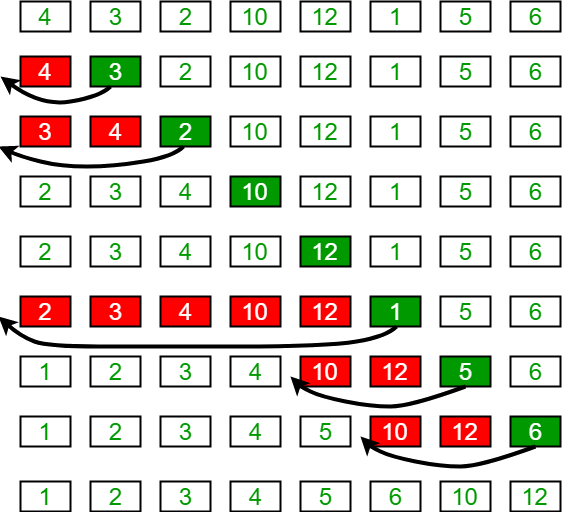
\includegraphics[height=0.6\paperheight]{imagens/insertion_sort.png}\\
	~ {\tiny Fonte: \url{https://www.geeksforgeeks.org/insertion-sort/}}
\end{figure}
\end{frame}

%-------------------------------------------------------
\begin{frame}\frametitle{\emph{Insertion Sort}: Exemplo 2}
\begin{center}
\begin{tabular}{CCCCCCCCCC}
\tiny{0} & \tiny{1} & \tiny{2} & \tiny{3} & \tiny{4} & \tiny{5} & \tiny{6} & \tiny{7} & \tiny{8} & \tiny{9}\\
\hline
\multicolumn{1}{|C|}{\cellcolor{lime}5} & \multicolumn{1}{|C|}{\cellcolor{yellow}7} & \multicolumn{1}{|C|}{8} & \multicolumn{1}{|C|}{1} & \multicolumn{1}{|C|}{10} & \multicolumn{1}{|C|}{9} & \multicolumn{1}{|C|}{4} & \multicolumn{1}{|C|}{6} & \multicolumn{1}{|C|}{3} & \multicolumn{1}{|C|}{2}\\
\hline
\hline
\multicolumn{1}{|C|}{\cellcolor{lime}5} & \multicolumn{1}{|C|}{\cellcolor{lime}7} & \multicolumn{1}{|C|}{\cellcolor{yellow}8} & \multicolumn{1}{|C|}{1} & \multicolumn{1}{|C|}{10} & \multicolumn{1}{|C|}{9} & \multicolumn{1}{|C|}{4} & \multicolumn{1}{|C|}{6} & \multicolumn{1}{|C|}{3} & \multicolumn{1}{|C|}{2}\\
\hline
\hline
\multicolumn{1}{|C|}{\cellcolor{lime}5} & \multicolumn{1}{|C|}{\cellcolor{lime}7} & \multicolumn{1}{|C|}{\cellcolor{lime}8} & \multicolumn{1}{|C|}{\cellcolor{yellow}1} & \multicolumn{1}{|C|}{10} & \multicolumn{1}{|C|}{9} & \multicolumn{1}{|C|}{4} & \multicolumn{1}{|C|}{6} & \multicolumn{1}{|C|}{3} & \multicolumn{1}{|C|}{2}\\
\hline
\hline
\multicolumn{1}{|C|}{\cellcolor{lime}1} & \multicolumn{1}{|C|}{\cellcolor{lime}5} & \multicolumn{1}{|C|}{\cellcolor{lime}7} & \multicolumn{1}{|C|}{\cellcolor{lime}8} & \multicolumn{1}{|C|}{\cellcolor{yellow}10} & \multicolumn{1}{|C|}{9} & \multicolumn{1}{|C|}{4} & \multicolumn{1}{|C|}{6} & \multicolumn{1}{|C|}{3} & \multicolumn{1}{|C|}{2}\\
\hline
\hline
\multicolumn{1}{|C|}{\cellcolor{lime}1} & \multicolumn{1}{|C|}{\cellcolor{lime}5} & \multicolumn{1}{|C|}{\cellcolor{lime}7} & \multicolumn{1}{|C|}{\cellcolor{lime}8} & \multicolumn{1}{|C|}{\cellcolor{lime}10} & \multicolumn{1}{|C|}{\cellcolor{yellow}9} & \multicolumn{1}{|C|}{4} & \multicolumn{1}{|C|}{6} & \multicolumn{1}{|C|}{3} & \multicolumn{1}{|C|}{2}\\
\hline
\hline
\multicolumn{1}{|C|}{\cellcolor{lime}1} & \multicolumn{1}{|C|}{\cellcolor{lime}5} & \multicolumn{1}{|C|}{\cellcolor{lime}7} & \multicolumn{1}{|C|}{\cellcolor{lime}8} & \multicolumn{1}{|C|}{\cellcolor{lime}9} & \multicolumn{1}{|C|}{\cellcolor{lime}10} & \multicolumn{1}{|C|}{\cellcolor{yellow}4} & \multicolumn{1}{|C|}{6} & \multicolumn{1}{|C|}{3} & \multicolumn{1}{|C|}{2}\\
\hline
\hline
\multicolumn{1}{|C|}{\cellcolor{lime}1} & \multicolumn{1}{|C|}{\cellcolor{lime}4} & \multicolumn{1}{|C|}{\cellcolor{lime}5} & \multicolumn{1}{|C|}{\cellcolor{lime}7} & \multicolumn{1}{|C|}{\cellcolor{lime}8} & \multicolumn{1}{|C|}{\cellcolor{lime}9} & \multicolumn{1}{|C|}{\cellcolor{lime}10} & \multicolumn{1}{|C|}{\cellcolor{yellow}6} & \multicolumn{1}{|C|}{3} & \multicolumn{1}{|C|}{2}\\
\hline
\hline
\multicolumn{1}{|C|}{\cellcolor{lime}1} & \multicolumn{1}{|C|}{\cellcolor{lime}4} & \multicolumn{1}{|C|}{\cellcolor{lime}5} & \multicolumn{1}{|C|}{\cellcolor{lime}6} & \multicolumn{1}{|C|}{\cellcolor{lime}7} & \multicolumn{1}{|C|}{\cellcolor{lime}8} & \multicolumn{1}{|C|}{\cellcolor{lime}9} & \multicolumn{1}{|C|}{\cellcolor{lime}10} & \multicolumn{1}{|C|}{\cellcolor{yellow}3} & \multicolumn{1}{|C|}{2}\\
\hline
\hline
\multicolumn{1}{|C|}{\cellcolor{lime}1} & \multicolumn{1}{|C|}{\cellcolor{lime}3} & \multicolumn{1}{|C|}{\cellcolor{lime}4} & \multicolumn{1}{|C|}{\cellcolor{lime}5} & \multicolumn{1}{|C|}{\cellcolor{lime}6} & \multicolumn{1}{|C|}{\cellcolor{lime}7} & \multicolumn{1}{|C|}{\cellcolor{lime}8} & \multicolumn{1}{|C|}{\cellcolor{lime}9} & \multicolumn{1}{|C|}{\cellcolor{lime}10} & \multicolumn{1}{|C|}{\cellcolor{yellow}2}\\
\hline
\hline
\multicolumn{1}{|C|}{\cellcolor{green}1} & \multicolumn{1}{|C|}{\cellcolor{green}2} & \multicolumn{1}{|C|}{\cellcolor{green}3} & \multicolumn{1}{|C|}{\cellcolor{green}4} & \multicolumn{1}{|C|}{\cellcolor{green}5} & \multicolumn{1}{|C|}{\cellcolor{green}6} & \multicolumn{1}{|C|}{\cellcolor{green}7} & \multicolumn{1}{|C|}{\cellcolor{green}8} & \multicolumn{1}{|C|}{\cellcolor{green}9} & \multicolumn{1}{|C|}{\cellcolor{green}10}\\
\hline
\end{tabular}
\end{center}
\end{frame}

%-------------------------------------------------------
\begin{frame}\frametitle{\emph{Insertion Sort}: Implementação}
\lstinputlisting{src/insertionSort.cpp}
\end{frame}

%-------------------------------------------------------
\begin{frame}[fragile]\frametitle{\emph{Insertion Sort}: Mais informações [*]}
\begin{itemize}
	\item \url{http://www.sorting-algorithms.com/insertion-sort}
	\item \url{https://www.hackerearth.com/practice/algorithms/sorting/insertion-sort/tutorial/}
\end{itemize}
\end{frame}

%=======================================================
\section{\emph{Merge Sort}}

%-------------------------------------------------------
\begin{frame}\frametitle{\emph{Merge Sort}}
\begin{itemize}
	\item É um algorimo de ordenação por intercalação
	\item Utiliza o padrão (estratégia) conhecido como ``divisão e conquista''
	\item Consiste de 3 etapas
	\begin{itemize}
		\item Divisão: se há algo a ordenar, divide os dados de entrada em duas (ou mais) partes e executa o algoritmo sobre cada uma das partes; se não há nada a ordenar, retorna a solução
		\item Conquista: cada parte dos dados é classificada recursivamente
		\item Combinação: quando cada subconjunto está classificado (internamente), eles devem ser combinados (\emph{merge}) realizando-se uma intercalação
	\end{itemize}
	\item Permite implementação recursiva
\end{itemize}
\end{frame}

%-------------------------------------------------------
\begin{frame}\frametitle{\emph{Merge Sort}: Estratégia [*]}
\begin{itemize}
	\item  Para ordenar uma sequência $S$ com $n$ elementos:
	\begin{itemize}
		\item \textbf{Dividir}: se $S$ tem zero ou um elemento, retorna $S$, pois já está classificado; senão, remove os elementos de $S$ e coloca-os em duas sequências, $S_1$ e $S_2$ ($n/2$ elementos em cada um)
		\item \textbf{Conquistar}: classifica as sequências $S_1$ e $S_2$ recursivamente
		\item \textbf{Combinar}: coloca os elementos de volta em $S$ com a união das sequências $S_1$ e $S_2$ ordenadas
	\end{itemize}
	\end{itemize}
\end{frame}

%-------------------------------------------------------
\begin{frame}\frametitle{\emph{Merge Sort}: Exemplo}
\begin{columns}[T]
\begin{column}{0.6\linewidth}
\vspace{-3mm}
\begin{figure}[h]
	\centering
	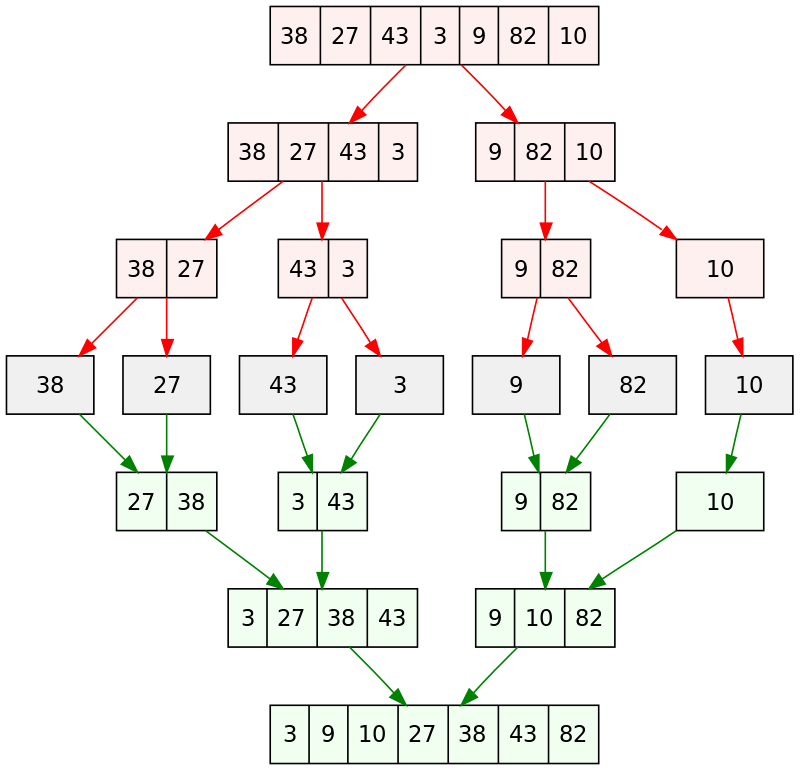
\includegraphics[height=0.7\paperheight]{imagens/mergesort.png}\\
	\tiny{Fonte: \url{https://en.wikipedia.org/wiki/Merge_sort}}
\end{figure}
\end{column}
\begin{column}{0.4\linewidth}
\vspace{3mm}
\begin{itemize}
	\item A execução do algoritmo pode ser vista como uma árvore binária
	\item Cada nodo representa uma chamada recursiva do algoritmo \emph{Merge Sort}
	\item Nodos recebem sequências de entrada para serem processadas e, por fim, geram sequências de saída ordenadas
\end{itemize}
\end{column}
\end{columns}
\end{frame}

%-------------------------------------------------------
\begin{frame}\frametitle{\emph{Merge Sort}: Implementação}
\lstinputlisting[basicstyle=\ttfamily\scriptsize]{src/mergeSort.cpp}
\end{frame}

%-------------------------------------------------------
\begin{frame}\frametitle{\emph{Merge Sort}: Desempenho [*]}
\begin{columns}[T]
\begin{column}{0.4\linewidth}
\vspace{3mm}
\begin{itemize}
	\item O tamanho da sequência de entrada é a metade a cada chamada recursiva
	\item A árvore associada a uma execução do algoritmo com uma sequência de tamanho $n$, tem altura $\log n$
	\item Conclusões:
	\begin{itemize}
		\item Altura da árvore é $\log n$
		\item Tempo gasto em cada nível: $O(n)$
		\item Tempo de execução: $O(n\log n)$
	\end{itemize}
\end{itemize}
\end{column}
\begin{column}{0.6\linewidth}
\vspace{-3mm}
\begin{figure}[h]
	\centering
	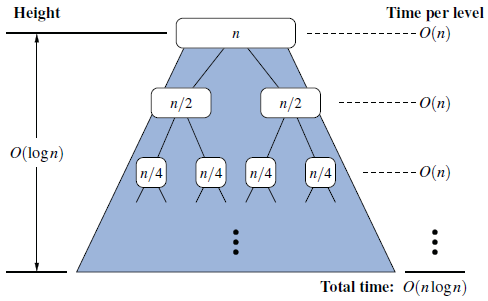
\includegraphics[height=0.6\paperheight]{imagens/mergesort_desempenho.png}
\end{figure}
\end{column}
\end{columns}
\end{frame}

%-------------------------------------------------------
\begin{frame}[fragile]\frametitle{\emph{Merge Sort}: Mais informações [*]}
\begin{itemize}
	\item \url{http://www.sorting-algorithms.com/merge-sort}
	\item \url{https://www.hackerearth.com/practice/algorithms/sorting/merge-sort/tutorial/}
\end{itemize}
\end{frame}

%=======================================================
\section{\emph{Quick Sort}}

%-------------------------------------------------------
\begin{frame}\frametitle{\emph{Quick Sort} [*]}
\begin{itemize}	
	\item Também utiliza o padrão ``Dividir para Conquistar'', mas de uma maneira diferente do \emph{Merge Sort}
	\item O maior processamento é feito \textbf{antes} das chamadas recursivas
	\item Estratégia geral:
	\begin{itemize}	
		\item Divisão de $S$ em subconjuntos (sequências)
		\item Recursão para classificar cada subconjunto
		\item Combinar as subsequências ordenadas através de uma concatenação simples
	\end{itemize}
\end{itemize}
\end{frame}

%-------------------------------------------------------
\begin{frame}\frametitle{\emph{Quick Sort}: 3 Etapas Principais [*]}
\begin{enumerate}
	\item Dividir
	\begin{itemize}	
		\item Se $S$ tem pelo menos dois elementos, seleciona um deles para ser o \textbf{pivô}
		\item O pivô pode ser qualquer elemento de $S$
		\item Remove todos os elementos de $S$ e coloca-os em três sequências:
		\begin{itemize}	
			\item $L$: armazena os elementos de $S$ menores que o pivô
			\item $E$: armazena os elementos de $S$ iguais ao pivô
			\item $G$: armazena os elementos de $S$ maiores que o pivô
		\end{itemize}
	\end{itemize}
	\item Conquistar
	\begin{itemize}	
		\item Recursivamente ordena as sequências $L$ e $G$
	\end{itemize}
	\item Combinar
	\begin{itemize}	
		\item  Coloca de volta os elementos em $S$, inserindo primeiro os elementos de $L$, depois de $E$ e finalmente de $G$
	\end{itemize}
\end{enumerate}
\end{frame}

%-------------------------------------------------------
\begin{frame}[fragile]\frametitle{\emph{Quick Sort}: Mais informações [*]}
\begin{itemize}
	\item \url{https://en.wikipedia.org/wiki/Quicksort}
	\item \url{http://www.sorting-algorithms.com/quick-sort}
	\item \url{https://www.hackerearth.com/practice/algorithms/sorting/quick-sort/tutorial/}
\end{itemize}
\end{frame}

\begin{comment}



Quick-sort
◼
 Execução do algoritmo pode ser vista como
uma árvore binária (quick-sort tree):
a)
 Sequência de entrada processada em cada nodo da
árvore
b)
 Sequência de saída gerada em cada nodo da árvore
Quick-sort
◼
 Execução do algoritmo pode ser vista como
uma árvore binária (quick-sort tree):
◼
 Altura pode chegar a ser linear
◼
 Por exemplo, quando a sequência consiste de n
elementos distintos já ordenados
◼
 L teria tamanho n-1, E tamanho 1 e G tamanho 0
◼
 A cada chamada do quick-sort para L, o tamanho
seria decrementado em 1, e a altura
da árvore seria n-1
Quick-sort
◼
 Execução do algoritmo quick-sort
◼
 Questões importantes:
◼
 Consumo de memória:
◼
 Na prática não são criados três vetores
◼
 O próprio vetor é alterado
◼
 Escolha do pivô



Quick-sort
◼
 Análise do tempo de execução do algoritmo
◼
 Tempo total de execução: O(n.h), sendo h a
altura da árvore
◼
 Pior caso: h = n-1, o que leva o tempo de
execução para O(n2)
Quick-sort
◼
 Análise do tempo de execução do algoritmo
◼
 O melhor para o quick-sort é quando L e G
possuem mais ou menos o mesmo tamanho
◼
 Neste caso, a árvore fica com altura O(log n) e o
tempo de execução do algoritmo fica O(n log n)
◼
 Escolher o último ou o primeiro elemento como
pivô se a sequência já está ordenada leva para
o pior caso
Quick-sort
◼
 Análise do tempo de execução do algoritmo
◼
 Solução:
◼
 Escolher o índice do pivô de forma randômica,
escolher o elemento do meio da sequência ou usar a
mediana de três valores (primeiro, meio e último)
◼
 Faz o quick-sort ter “na média” tempo de execução
O(n log n)
◼
 Tirando a escolha do pivô, o algoritmo permanece o
mesmo

\end{comment}

%=======================================================
\section{Comparação}

%-------------------------------------------------------
\begin{frame}[fragile]\frametitle{Estabilidade [*]}
\begin{itemize}	
	\item Um algoritmo de ordenação é estável (\emph{stable}) se não altera a posição relativa dos elementos que têm o mesmo valor
	\item Exemplo:
	\begin{itemize}
		\item Coleção inicial:
\begin{verbatim}
{ {"João", 21}, {"Ana", 55}, {"João", 13"}, {"Beto", 34}, {"Yuri", 23} }
\end{verbatim}
		\item Coleção ordenada por um algoritmo estável:
\begin{verbatim}
{ {"Ana", 55}, {"Beto", 34}, {"João", 21}, {"João", 13"}, {"Yuri", 23} }
\end{verbatim}
		\item Coleção ordenada por um algoritmo instável:
\begin{verbatim}
{ {"Ana", 55}, {"Beto", 34}, {"João", 13"}, {"João", 21}, {"Yuri", 23} }
\end{verbatim}
	\end{itemize}
\end{itemize}
\end{frame}

%-------------------------------------------------------
\begin{frame}\frametitle{Comparação dos Algoritmos quanto à Estabilidade}
\begin{itemize}	
	\item São estáveis:
	\begin{itemize}	
		\item \emph{Bubble Sort}
		\item \emph{Insertion Sort}
		\item \emph{Merge Sort}
	\end{itemize}
	\item São instáveis:
	\begin{itemize}	
		\item \emph{Selection Sort}
		\item \emph{Quick Sort}
	\end{itemize}
\end{itemize}
\end{frame}

%-------------------------------------------------------
\begin{frame}\frametitle{\emph{Bubble Sort}}
\begin{itemize}
	\item Complexidade: $O(n^2)$ (pior caso) ou $O(n)$ (melhor caso, considerando a implementação otimizada)
	\item Vantagens:
	\begin{itemize}	
		\item É simples de ser implementado
		\item É estável
		\item Não necessita de um vetor auxiliar (\emph{in-place}), ocupando menos memória
	\end{itemize}
	\item Desvantagens:
	\begin{itemize}	
		\item NÃO é recomendado para vetores grandes
		\item Executa SEMPRE $(n^2-n)/2$ comparações
	\end{itemize}
\end{itemize}
\end{frame}

%-------------------------------------------------------
\begin{frame}\frametitle{\emph{Selection Sort}}
\begin{itemize}
	\item Complexidade: $O(n^2)$
	\item Vantagens:
	\begin{itemize}	
		\item É simples de ser implementado
		\item Não necessita de um vetor auxiliar (\emph{in-place}), ocupando menos memória
		\item É relativamente rápido para pequenos vetores
	\end{itemize}
	\item Desvantagens:
	\begin{itemize}	
		\item É um dos mais lentos para vetores grandes
		\item NÃO é estável
		\item Executa SEMPRE $(n^2-n)/2$ comparações
	\end{itemize}
\end{itemize}
\end{frame}

%-------------------------------------------------------
\begin{frame}\frametitle{\emph{Insertion Sort}}
\begin{itemize}
	\item Complexidade: $O(n^2)$ (pior caso) ou $O(n)$ (melhor caso)
	\item Vantagens:
	\begin{itemize}	
		\item É estável
	\end{itemize}
	\item Desvantagens:
	\begin{itemize}	
		\item ...
	\end{itemize}
\end{itemize}
\end{frame}

%-------------------------------------------------------
\begin{frame}\frametitle{\emph{Merge Sort}}
\begin{itemize}
	\item Complexidade: $O(n\log{n})$
	\item Vantagens:
	\begin{itemize}	
		\item É estável
	\end{itemize}
	\item Desvantagens:
	\begin{itemize}	
		\item ...
	\end{itemize}
\end{itemize}
\end{frame}

%-------------------------------------------------------
\begin{frame}\frametitle{\emph{Quick Sort}}
\begin{itemize}
	\item Complexidade: $O(n\log{n})$
	\item Vantagens:
	\begin{itemize}
		\item ...
	\end{itemize}
	\item Desvantagens:
	\begin{itemize}	
		\item NÃO é estável
	\end{itemize}
\end{itemize}
\end{frame}

\begin{comment}

Comparação
◼
 Qual é o melhor algoritmo?
◼
 Não existe claramente o “melhor”
◼
 O algoritmo que melhor se aplica para um uso
específico depende de várias propriedades
◼
 Existem algumas “diretivas” e observações
◼
 Observação:
◼
 Algoritmo de ordenação é dito in-place se utiliza apenas
uma quantidade constante de memória, além daquela
necessária para os objetos, eles próprios ordenados



◼
 Insertion-sort
◼
 Se bem implementado, tempo de execução
pode ser O(n+k), sendo k o número de
inversões (pares de elementos fora de ordem)
◼
 Portanto
◼
 É simples de programar
◼
 É excelente para ordenar pequenas sequências (<50)
◼
 É bastante eficiente para ordenar sequências “quase”
ordenadas
◼
 Fora destas situações torna-se uma escolha pobre
pelo tempo de execução O(n2)


Comparação
◼
 Merge-sort
 Difícil de executar in-place
◼
 Torná-lo in-place exige um algoritmo mais complicado
◼
 Fica menos atrativo do que as implementações in-
place do quick-sort para sequências que cabem na
memória principal do computador
◼
 Sendo assim, é excelente para casos em que a
entrada não cabe na memória principal e precisa ser
armazenada em blocos em uma memória externa
◼
 Tende a minimizar os acessos a disco para fazer
leitura/escrita


Comparação
◼
 Quick-sort
◼
 Análises experimentais mostram que se a se-
quência de entrada couber na memória principal:
◼
 Versões in-place do quick-sort executam mais rápido
que o merge-sort
◼
 E o quick-sort tende, em média, a ser melhor que o
heap-sort
◼
 Então, é uma ótima escolha como algoritmo de
ordenação de finalidades genéricas no uso em
memória
◼
 Tempo O(n2) para o pior caso, torna-o uma
escolha pobre para aplicações em tempo real




%-------------------------------------------------------
\begin{frame}\frametitle{Exemplo clássico: Fatorial}
\begin{itemize}
	\item O fatorial de n é normalmente definido como:
\[ n! = \prod_{k=1}^{n}{k} = n \times (n-1) \times (n-2) \times ... \times 3 \times 2 \times 1,\qquad \forall n \in \mathbb{N}\]
	\item Por exemplo:
\[5 ! = 5 \times 4 \times 3 \times 2 \times 1 = 120\]
	\item Mas também pode-se usar a sua definição recursiva:
\[ n! = \begin{cases}
1, & \mbox{se ~ } n=0 \mbox{~ ou ~ } n=1\\
n \times (n-1)!, & \mbox{se ~ } n > 1
\end{cases} \]
\end{itemize}
\end{frame}

%-------------------------------------------------------
\begin{frame}[fragile]\frametitle{Implementação do Fatorial}
\begin{itemize}
	\item Iterativo
{\scriptsize\lstinputlisting{src/fatorial.cpp}}
	\item Recursivo
{\scriptsize\lstinputlisting{src/fatorialRec.cpp}}
\end{itemize}
\end{frame}

%-------------------------------------------------------
\begin{frame}\frametitle{Exemplo: Contagem}
\begin{itemize}
	\item Iterativo
{\scriptsize\lstinputlisting{src/contagem.cpp}}
	\pause
	\item Recursivo
{\scriptsize\lstinputlisting{src/contagemRec.cpp}}
\end{itemize}
\end{frame}

%-------------------------------------------------------
\begin{frame}\frametitle{Exercício: Contagem Regressiva}
\begin{itemize}
	\item Iterativo
{\scriptsize\lstinputlisting{src/contagemRegressiva.cpp}}
	\pause
	\item Recursivo
{\scriptsize\lstinputlisting{src/contagemRegressivaRec.cpp}}
\end{itemize}
\end{frame}

%-------------------------------------------------------
\begin{frame}\frametitle{Exercício: Geração de Índices de uma Matriz}
\begin{itemize}
	\item Iterativo
{\scriptsize\lstinputlisting{src/indicesMatriz.cpp}}
	\pause
	\item Recursivo
{\scriptsize\lstinputlisting{src/indicesMatrizRec1.cpp}}
	\pause
	\item \textbf{Desafio:} faça uma versão recursiva do algoritmo acima sem usar nenhum laço!
\end{itemize}
\end{frame}

%-------------------------------------------------------
\begin{frame}\frametitle{Recursividade [*]}
\begin{itemize}
	\item Poderosa ferramenta de programação
	\item Apesar de bastante empregada, nem sempre ela deve ser aplicada
	\begin{itemize}
		\item É preciso analisar o problema e ver se necessita de uma solução recursiva
	\end{itemize}
	\item Quando bem empregada pode tornar a solução de um problema clara, simples e consisa
\end{itemize}
\end{frame}

%-------------------------------------------------------
\begin{frame}\frametitle{Vantagens [*]}
\begin{itemize}
	\item Rotinas mais concisas
	\item Relação direta com uma prova por indução matemática
	\begin{itemize}
		\item Indução matemática: metodo de prova matemática usado para demonstrar a verdade de um número infinito de proposições
		\begin{itemize}
			\item Válida se funciona para $n$ igual a $0$ ou $1$
			\item Válida se vale para $n$ igual a $k$ e $k + 1$
		\end{itemize}
		\item Facilita verificar a correção
	\end{itemize}
\end{itemize}
\end{frame}

%-------------------------------------------------------
\begin{frame}\frametitle{Desvantagens [*]}
\begin{itemize}
	\item Cada chamada recursiva implica em um custo (tempo e espaço)
	\begin{itemize}
		\item Informações são armazenadas na pilha
		\item Para cada chamada realizada, um conjunto de variáveis locais é alocado (criado)
		\item Cada chamada requer
		\begin{itemize}
			\item O empilhamento de parâmetros e endereços de retorno da função que chama
			\item A alocação de variáveis locais da função % [Roland]
			%\item O desempilhamento de parâmetros pela função que executa
		\end{itemize}
		\item Cada retorno requer
		\begin{itemize}
			\item A desalocação das variáveis locais da função % [Roland]
			\item O desempilhamento do endereço de retorno
			%\item O empilhamento do resultado (ou passagem por registrador)
			%\item O desempilhamento do retorno pela função que chamou
		\end{itemize}
	\end{itemize}
\end{itemize}
\end{frame}

%=======================================================
\section{Algoritmos de Pesquisa}

%-------------------------------------------------------
\begin{frame}\frametitle{Algoritmos de Pesquisa}
\begin{itemize}
	\item Localizam um elemento dentro de uma coleção
	\item Podem retornar
	\begin{itemize}
		\item \textbf{Valor booleano} (\texttt{true} se o elemento existir na coleção ou \texttt{false}, em caso contrário) ou
		\item \textbf{Índice} (posição) do elemento na coleção (ou -1 se não encontrar)
	\end{itemize}
	\item Para coleções \textbf{desordenadas}, deve-se usar um algoritmo de \textbf{pesquisa linear}
	\item Quando a coleção está \textbf{ordenada}, pode-se usar um algoritmo de \textbf{pesquisa binária}
\end{itemize}
\end{frame}

%-------------------------------------------------------
\begin{frame}\frametitle{Pesquisa Linear}
\begin{itemize}
	\item Serve para coleções \textbf{desordenadas}
	\item Estratégia: comparar o elemento procurado com cada item da coleção até encontrar ou até chegar ao fim
	\item Melhor caso: o elemento procurado é o primeiro da lista
	\item Pior caso: o elemento procurado \textbf{NÃO} existe na lista
	\item Também poderia ser aplicado sobre coleções ordenadas
	\pause
	\item Complexidade: $O(n)$
\end{itemize}
\end{frame}

%-------------------------------------------------------
\begin{frame}[fragile]\frametitle{Implementação da Pesquisa Linear}
\begin{itemize}
	\item Iterativo
{\scriptsize\lstinputlisting{src/pesquisaLinear.cpp}}
	\pause
	\item Recursivo
{\scriptsize\lstinputlisting{src/pesquisaLinearRec.cpp}}
\end{itemize}
\end{frame}

%-------------------------------------------------------
\begin{frame}\frametitle{Pesquisa Binária}
\begin{itemize}
	\item Serve \textbf{APENAS} para coleções \textbf{ordenadas}
	\item Estratégia:
	\begin{itemize}
		\item Compara o valor procurado com o elemento do meio
		\begin{itemize}
			\item Se for igual, encontrou
			\item Se for menor, continua-se a busca na metade inferior (desconsidera a metade superior)
			\item Se for maior, continua-se a busca na metade superior (desconsidera a metade inferior)
		\end{itemize}
		\item Repete-se o procecimento até que o valor procurado seja encontrado ou até que não se consiga dividir a coleção
	\end{itemize}
	\pause
		\item Complexidade: $O(\log{n})$
\end{itemize}
\end{frame}

%-------------------------------------------------------
\begin{frame}[fragile]\frametitle{Pesquisa Binária Iterativa}
\lstinputlisting[basicstyle=\ttfamily\scriptsize]{src/pesquisaBinaria.cpp}
\end{frame}

%-------------------------------------------------------
\begin{frame}\frametitle{Pesquisa Binária: Exemplo (\texttt{valor = 18})}
\begin{itemize}

	\item Passo 1:
\begin{tabular}{cccccccccc}
\tiny{0} & \tiny{1} & \tiny{2} & \tiny{3} & \tiny{4} & \tiny{5} & \tiny{6} & \tiny{7} & \tiny{8} & \tiny{9}\\
\hline
\multicolumn{1}{|c|}{2} & \multicolumn{1}{c|}{4} & \multicolumn{1}{c|}{6} & \multicolumn{1}{c|}{8} & \multicolumn{1}{c|}{10} & \multicolumn{1}{c|}{12} & \multicolumn{1}{c|}{14} & \multicolumn{1}{c|}{16} & \multicolumn{1}{c|}{18} & \multicolumn{1}{c|}{20}\\
\hline
$\uparrow$ & & & & $\uparrow$ & & & & & $\uparrow$ \\
{\tiny\texttt ini} & & & & {\tiny\texttt meio} & & & & & {\tiny\texttt fim} \\
\end{tabular}

	\item Passo 2:
\begin{tabular}{cccccccccc}
\tiny{0} & \tiny{1} & \tiny{2} & \tiny{3} & \tiny{4} & \tiny{5} & \tiny{6} & \tiny{7} & \tiny{8} & \tiny{9}\\
\hline
\multicolumn{1}{|c|}{2} & \multicolumn{1}{c|}{4} & \multicolumn{1}{c|}{6} & \multicolumn{1}{c|}{8} & \multicolumn{1}{c|}{10} & \multicolumn{1}{c|}{12} & \multicolumn{1}{c|}{14} & \multicolumn{1}{c|}{16} & \multicolumn{1}{c|}{18} & \multicolumn{1}{c|}{20}\\
\hline
 & & & & & $\uparrow$ & & $\uparrow$ & & $\uparrow$ \\
 & & & & & {\tiny\texttt ini} & & {\tiny\texttt meio} & & {\tiny\texttt fim} \\
\end{tabular}

	\item Passo 3:
\begin{tabular}{cccccccccc}
\tiny{0} & \tiny{1} & \tiny{2} & \tiny{3} & \tiny{4} & \tiny{5} & \tiny{6} & \tiny{7} & \tiny{8} & \tiny{9}\\
\hline
\multicolumn{1}{|c|}{2} & \multicolumn{1}{c|}{4} & \multicolumn{1}{c|}{6} & \multicolumn{1}{c|}{8} & \multicolumn{1}{c|}{10} & \multicolumn{1}{c|}{12} & \multicolumn{1}{c|}{14} & \multicolumn{1}{c|}{16} & \multicolumn{1}{c|}{18} & \multicolumn{1}{c|}{20}\\
\hline
 & & & & & & & & $\uparrow$ & $\uparrow$ \\
 & & & & & & & & {\tiny\texttt ini} & {\tiny\texttt fim} \\
 & & & & & & & & {\tiny\texttt meio} & \\
\end{tabular}
 ~ Valor 18 encontrado no índice 8!
\end{itemize}
\end{frame}

%-------------------------------------------------------
\begin{frame}\frametitle{Pesquisa Binária: Exemplo (\texttt{valor = 5})}
\begin{itemize}

	\item Passo 1:
\begin{tabular}{cccccccccc}
\tiny{0} & \tiny{1} & \tiny{2} & \tiny{3} & \tiny{4} & \tiny{5} & \tiny{6} & \tiny{7} & \tiny{8} & \tiny{9}\\
\hline
\multicolumn{1}{|c|}{2} & \multicolumn{1}{c|}{4} & \multicolumn{1}{c|}{6} & \multicolumn{1}{c|}{8} & \multicolumn{1}{c|}{10} & \multicolumn{1}{c|}{12} & \multicolumn{1}{c|}{14} & \multicolumn{1}{c|}{16} & \multicolumn{1}{c|}{18} & \multicolumn{1}{c|}{20}\\
\hline
$\uparrow$ & & & & $\uparrow$ & & & & & $\uparrow$ \\
{\tiny\texttt ini} & & & & {\tiny\texttt meio} & & & & & {\tiny\texttt fim} \\
\end{tabular}\\~\\~

	\item Passo 2:
\begin{tabular}{cccccccccc}
\tiny{0} & \tiny{1} & \tiny{2} & \tiny{3} & \tiny{4} & \tiny{5} & \tiny{6} & \tiny{7} & \tiny{8} & \tiny{9}\\
\hline
\multicolumn{1}{|c|}{2} & \multicolumn{1}{c|}{4} & \multicolumn{1}{c|}{6} & \multicolumn{1}{c|}{8} & \multicolumn{1}{c|}{10} & \multicolumn{1}{c|}{12} & \multicolumn{1}{c|}{14} & \multicolumn{1}{c|}{16} & \multicolumn{1}{c|}{18} & \multicolumn{1}{c|}{20}\\
\hline
$\uparrow$ & $\uparrow$ & & $\uparrow$ & & & & & & \\
{\tiny\texttt ini} & {\tiny\texttt meio}& & {\tiny\texttt fim} & & & & & & \\
\end{tabular}

\end{itemize}
\end{frame}

%-------------------------------------------------------
\begin{frame}\frametitle{Pesquisa Binária: Exemplo (\texttt{valor = 5})}
\begin{itemize}

	\item Passo 3:
\begin{tabular}{cccccccccc}
\tiny{0} & \tiny{1} & \tiny{2} & \tiny{3} & \tiny{4} & \tiny{5} & \tiny{6} & \tiny{7} & \tiny{8} & \tiny{9}\\
\hline
\multicolumn{1}{|c|}{2} & \multicolumn{1}{c|}{4} & \multicolumn{1}{c|}{6} & \multicolumn{1}{c|}{8} & \multicolumn{1}{c|}{10} & \multicolumn{1}{c|}{12} & \multicolumn{1}{c|}{14} & \multicolumn{1}{c|}{16} & \multicolumn{1}{c|}{18} & \multicolumn{1}{c|}{20}\\
\hline
 & & $\uparrow$ & $\uparrow$ & & & & & & \\
 & & {\tiny\texttt ini} & {\tiny\texttt fim} & & & & & & \\
 & & {\tiny\texttt meio} & & & & & & & \\
\end{tabular}\\~\\~

	\item Passo 4:
\begin{tabular}{cccccccccc}
\tiny{0} & \tiny{1} & \tiny{2} & \tiny{3} & \tiny{4} & \tiny{5} & \tiny{6} & \tiny{7} & \tiny{8} & \tiny{9}\\
\hline
\multicolumn{1}{|c|}{2} & \multicolumn{1}{c|}{4} & \multicolumn{1}{c|}{6} & \multicolumn{1}{c|}{8} & \multicolumn{1}{c|}{10} & \multicolumn{1}{c|}{12} & \multicolumn{1}{c|}{14} & \multicolumn{1}{c|}{16} & \multicolumn{1}{c|}{18} & \multicolumn{1}{c|}{20}\\
\hline
 & $\uparrow$ & $\uparrow$ & & & & & & & \\
 & {\tiny\texttt fim} & {\tiny\texttt ini} & & & & & & & \\
\end{tabular}
 ~ Valor 5 \textbf{NÃO} encontrado!

\end{itemize}
\end{frame}

%-------------------------------------------------------
\begin{frame}[fragile]\frametitle{Pesquisa Binária Recursiva}
\lstinputlisting[basicstyle=\ttfamily\scriptsize]{src/pesquisaBinariaRec.cpp}
\end{frame}

%=======================================================
\section{Exercícios}

%-------------------------------------------------------
\begin{frame}\frametitle{Exercícios}
\begin{enumerate}
	\item Dado um valor inteiro e positivo (\texttt{n}), o valor da constante de \emph{Euler} poder ser calculando com precisão diretamente proporcional a \texttt{n} através da fórmula:
\[ E = \frac{1}{0!} + \frac{1}{1!} + \frac{1}{2!}+ \frac{1}{3!} + ... + \frac{1}{n!}\]
Implemente, em C, um método recursivo que recebe \texttt{n}, retornando o valor de \emph{Euler} calculado usando a fórmula acima.
	\item Considere a função abaixo, que implementa o somatório de um vetor e implemente a sua versão recursiva.
\lstinputlisting[basicstyle=\ttfamily\tiny]{src/somatorio.cpp}
\end{enumerate}
\end{frame}

%-------------------------------------------------------
\begin{frame}\frametitle{Exercícios}
\begin{enumerate}
        \setcounter{enumi}{2}
	\item Considere a função que implementa o algoritmo \emph{Bubble Sort} (apresentada na unidade anterior) e implemente a sua versão recursiva).
	\item Implemente uma função recursiva que inverte os elementos de um vetor, trocando o primeiro elemento com o último, o segundo com o penúltimo, e assim sucessivamente.
	\item Implemente uma função recursiva que verifica se uma cadeia de caracteres recebida como parâmetro é um palíndromo ou não. Por exemplo, ``socorrammesubinoonibusemmarrocos'' é um palíndromo.
	%\item Faça o algoritmo da potência de forma não recursiva e de forma recursiva. Considere que o valor da base e do expoente são recebidos por parâmetro, inteiros e positivos.
\end{enumerate}
\end{frame}

%=======================================================
\section{Soluções}

%-------------------------------------------------------
\begin{frame}\frametitle{Soluções}
\begin{enumerate}
	\item \lstinputlisting[basicstyle=\ttfamily\tiny]{src/eulerRec.cpp}

	\item \lstinputlisting[basicstyle=\ttfamily\tiny]{src/somatorioRec.cpp}

	\item \lstinputlisting[basicstyle=\ttfamily\tiny]{src/bubbleSortRec.cpp}
\end{enumerate}
\end{frame}

%-------------------------------------------------------
\begin{frame}\frametitle{Soluções}
\begin{enumerate}
        \setcounter{enumi}{3}
	\item \lstinputlisting[basicstyle=\ttfamily\tiny]{src/inverteVetorRec.cpp}

	\item \lstinputlisting[basicstyle=\ttfamily\tiny]{src/palindromoRec.cpp}

\end{enumerate}
\end{frame}

\end{comment}

%=======================================================
\section{Créditos}

%-------------------------------------------------------
\begin{frame}\frametitle{Créditos}
\begin{itemize}
	\item Estas lâminas contêm trechos adaptados de materiais criados e disponibilizados pela professora Isabel Harb Manssour [*].
\end{itemize}
\end{frame}

%-------------------------------------------------------
\end{document}

